	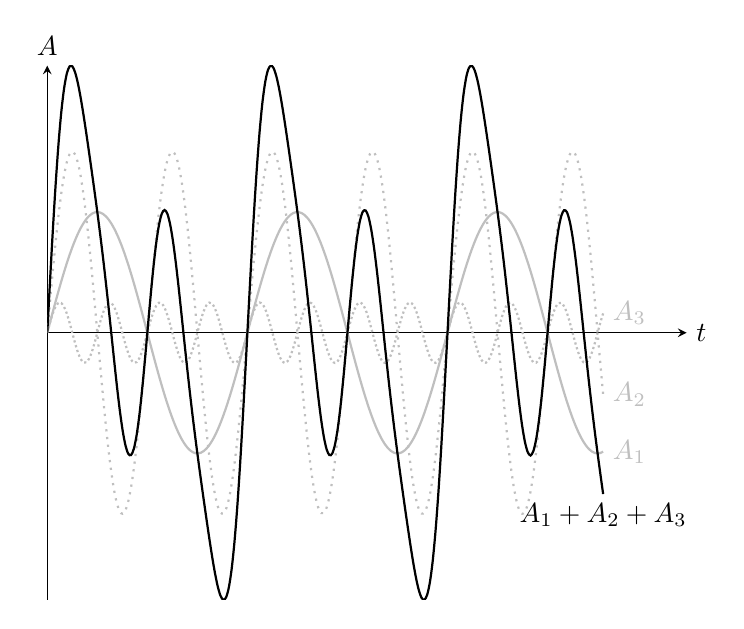
\begin{tikzpicture}[domain = 0:16, samples = 1000]
		%\draw[very thin, color = gray, step=1] (0,-2.75) grid(16,2.75);
		% zero crossing
		%\draw[dotted] (0,0) -- (16,0);
		%\draw (6.25,3) -- (6.25,-3) node[below] {$4ms$};
		\begin{axis}[
			width = 0.8\textwidth,
			axis x line=middle,
			axis y line=middle,
			ylabel = {$A$},
			ylabel style={at=(current axis.above origin), anchor=south}, 
			ytick=\empty,
			xtick=\empty,
				xlabel = {$t$},
				xlabel style={at=(current axis.right of origin), anchor=west},
				xmax=1150]	
		%	height = 0.5\textwidth]
		\addplot[thick, dotted, color=lightgray,
		domain = 0:1000,
		samples = 200,
		smooth]
	{sin(2*x)*1.5} node (b){};
	\node [right,color=lightgray] at (b) {$A_2$};
		\addplot[thick, color=lightgray,domain = 0:1000,
		samples = 200,
		smooth] plot[id=a]
	{sin(x)} node (a){};
	\node [right,color=lightgray] at (a) {$A_1$};
		\addplot[thick, color=lightgray, densely dotted,domain = 0:1000,
		samples = 200,
		smooth] plot[id=b]
	{sin(4*x)/4} node (c){};
	\node [right,color=lightgray] at (c) {$A_3$};
		\addplot[thick,id =d,domain = 0:1000,
		samples = 200,
		smooth]	{sin(4*x)/4 + sin(x) +  sin(2*x)*1.5}  node (y){};
		\node [below] at (y) {$A_1 + A_2 + A_3$};

\end{axis}
	\end{tikzpicture}
